% file: reasoning_case.tex

\begin{ReasoningBox}[title=Numerical Reasoning] % 可以通过 title 参数修改标题
    % --- 第一部分：问题描述与图片 ---
    % \begin{minipage}[t]{0.58\textwidth}
    \begin{wrapfigure}{r}{0.3\textwidth}
        \centering
        % wrapfigure 通常顶部会有多余空白，使用负 vspace 向上提，让图片和第一行文字对齐
        \vspace{-20pt} 
        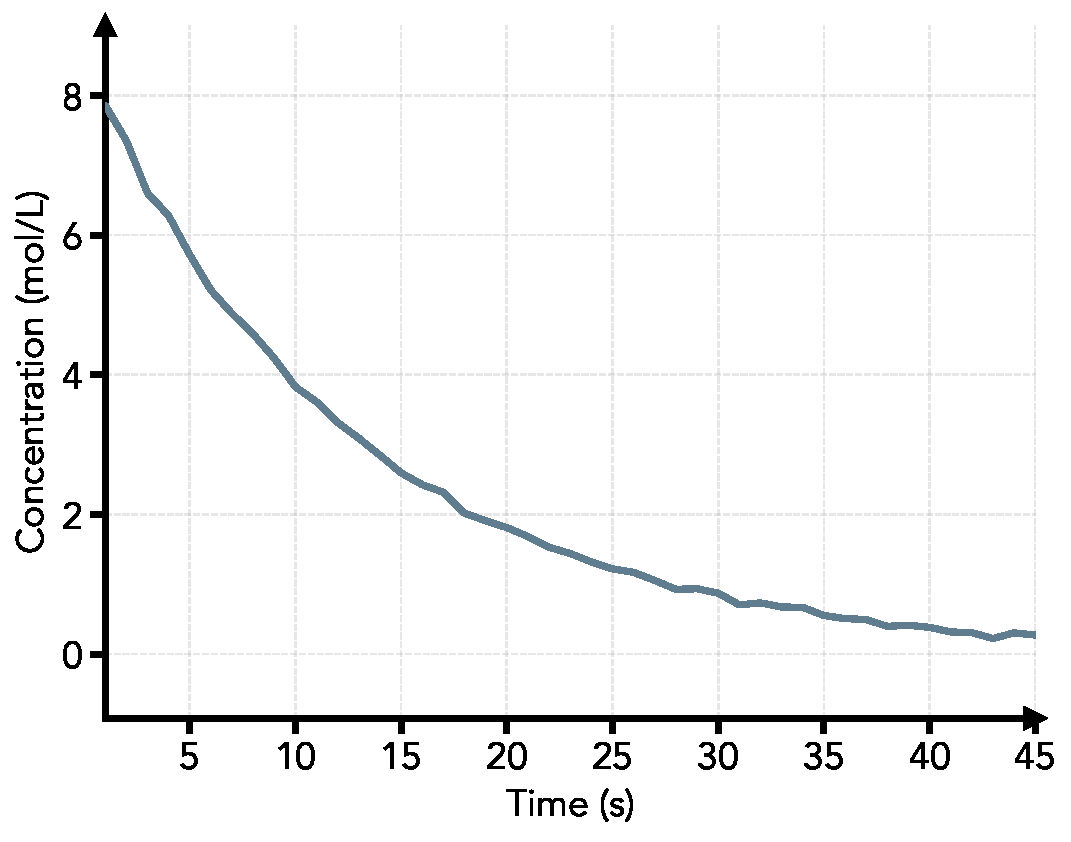
\includegraphics[width=\linewidth]{blocks/sample_cases_success/numerical.pdf}
        % 调整底部的留白
        \vspace{-20pt}
    \end{wrapfigure}
        \textbf{Question:} The following time series shows the concentration (in mol/L) of a reactant over time during a chemical reaction. 
Based on the concentration decay pattern, determine the reaction order (zero, first, or second) and calculate the 
rate constant $k$. For zero-order: $C = C_0 - kt$; for first-order: $C = C_0 e^{-kt}$; for second-order: 
$\frac{1}{C} = \frac{1}{C_0} + kt$. 

Assume this is a first-order reaction and calculate $k$.


    \vspace{0.5em}

    % --- 第二部分：选项 ---
    \textbf{Answer Choices:} \\ (A) 2.064 \\ (B) 0.0344 \\ (C) 0.0241 \\ (D) 0.0758 \\
    \textbf{Correct Answer:} \textcolor{correctgreen}{(B)} \\
\end{ReasoningBox}